\chapter{Research Methodology}

\section{Overview}
This chapter highlights the employed methods of how research was conducted during this project. This includes an overall description of what has been done, followed by an in depth description of each element employed within the project. The individual elements include my collected metrics, tasks given to study participants, how participants were recruited and how they are categorised into Novice and Experienced categories.

\section{Research Methods and Planning}
\subsection{Experiment Procedures}
To begin this project, participants were asked to complete a short pre-study questionnaire (see Appendix B.3), this was to collected basic details and to categorise participants into Novice and Experienced users of gaming services such as Steam. A series of series of individual study sessions were then conducted, lasting around 20-30 minutes per participant. During each session the necessary materials were given to each participant, this included the reasons for the study, any risks of the study to the participant, what data that was to be collected and how it was collected. This included recording the participants voice and the laptop screen for the duration of the experiment using OBS (Open Broadcast Software \citep{OBS2019}) and a microphone (see Appendix B.2). Any questions were answered before the beginning of each session, if the participant had any queries, clarifying that any questions asked during the experiment would not be answered such as how to infer or even complete the six tasks describes further below. Participants were then asked to begin from Task A and sequentially attempt each of the tasks in turn. Once a task was completed the task completion time, whether the task was completed with the expected outcome, the number of mouse interactions and finally any errors, issues or relevant comments made by each participant were recorded using materials seen in Appendix B as they attempted each Task. Due to the recorded data taken via OBS, it was possible to refer back to video and audio logs to confirm any further issues that may have been missed during each session. Conditions were made to be as similar as possible for each test session using a quiet location as well as limiting a number of distractions as possible, equipment and software was prepared the same way for each participant session. The laptop display was 15.6 inches across and in the same brightness settings, a wireless mouse was also provided to be used in the test sessions instead of the laptops track-pad, to provide better ergonomics for the participants in this test and remove the factor of unforgettable study materials influencing the participants. Initially this study was to have  40 participants in total, split into two even groups. However this study involved total of 32 participants, as the process of organising and conducting each study experiment was more time consuming then first considered. It was also challenging to find an equal split in each groups demographics especially with regards to age, which shall be discussed more  Chapter 6 Research Discussion. 

\subsection{Role of the Observer}
During the experiments the Practitioners involvement was as minimal as possible. This was to reduce the potential influence that could have been had upon both types of  participants, although Novice users would likely have been more influenced due to the unfamiliar nature of the tested program. For instance, any questions that the participants had whilst the sessions were happening were not answered. This was to ensure the participant was not influenced in how to proceed with each task. For instance a question such as ``Is this correct?" or ``Am I doing this right?", could not be answered as if a positive or negative response was given to the participant it would likely have changed their actions based on the response and thus contribute to the collection of altered results \citep{alhadreti2016thinking}. Therefore When asked such questions, neutral responds were given and the task continued onward.

\section{Tasks for Participants}
The Steam client was installed onto the testing laptop which all participants used, alongside the same mouse and microphone. A new Steam account was prepared in the following ways; three games that were available on the service were purchased, two of these games where already installed (Hollow Knight, Sid Meier's Civilization 5), and the third uninstalled, Terraria. This was because Terraria was part of Task B which was to try to install a pre-purchased game within the test accounts library. Below are the six tasks that participants were asked to attempt during the study, further illustrated details can be be seen in Appendix B.6. Additionally in Appendix A I have several screen shots from the Steam Client which provide some context to these tasks. Figures 2, 3 and 4 relate to Task A, figures 5 and 6 for Task B, figures 7,8 and 9 for Task C, figures 10, 11 and 12 for Task D, figures 13 and 14 for Task E and finally figures 15, 16 and 17 for Task F. The purpose of these figures is to give a walk through of what an experienced user would do to complete all Tasks successfully, the images are not exact emulators of the Tasks given to the participants, as games were different, but the process of the Task remained the same.

\begin{figure}[H]
    \centering
    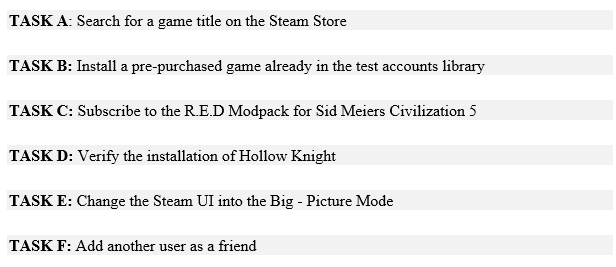
\includegraphics{Screenshots/StudyMaterialScreenshots/tasklist.png}
\end{figure} 

Task A required participants to search the Steam store for a game title, and then subsequently display the store page for the searched game. This task is one of the most common tasks that a Steam user can do, as this is the main service that Valve offers, aside from playing the purchased game which is not a task featured in this study. Additionally the way task is present in a multitude of applications and as such I foresaw that there would not be a huge number of issues or errors from this task, as it is in essence searching a database, which in this case is full of games. 

Task B asked my participants too install a pre-purchased game which is in the test accounts library. This task is relatively common for Steam users, especially if they are installing Steam onto a new PC or laptop, or if they are having issues with a game that requires an re-installation to fix. This task is more complex than task A, but is still relatively straight forward and again I expect fewer issues encountered by both sets of participants, especially those in the experienced category. Experienced participants are likely used to this concept on there respective platforms outside of Steam, such as using a gaming console.  

Task C involved using the Steam Workshop which is an aspect of Steam which community developed modifications available for a large number of titles on the Steam service. This task is the most difficult task of the six. Firstly, many of the participants are unlikely to be familiar with the concepts of modifications in relation to gaming, additionally it is also task that requires multiple interactions on different pages within the Steam client, thus heightening the possibility that participants could become lost within the service. There are also a multitude of different modifications available which could cause some further confusion, especially for Novice participants. However I also expected that Experienced participants would encounter difficulties, as many gaming users do not have an interest in modifying there purchases, and just wish to enjoy the product they purchased as the developers intended.

Task D is another somewhat difficult task. The process of verification involves taking an already installed game and checking that all files that are expected are present within the installation directory. This can be useful for Steam users as many games are hundreds of gigabytes in size and therefore re-installing all of the game data can be extremely time consuming, especially if the user does not have a strong internet connection. Therefore by using verification this can be avoided. However in order to achieve this, a user must find the corresponding properties menu for the game in question, which involves a right-click on the particular game. However this is not sign-posted as can be easily missed, which I again expected many participants of both types to encounter.  

Task E involved changing the \gls{ui} of the Steam Client so that it become more convenient for users who prefer a more console like experience, known as \gls{bpm}. This refers to using a Xbox Controller in order to play games as one example, and therefore forgoing the use of keyboard and mouse as an input method. The \gls{ui} is changed so that visual elements are far larger and can be seen a a greater distance, suitable for use on a large television. Changing to this mode is not extremely difficult and can be achieved in one button press, however due to the unfamiliar terminology I expected some participants to encounter problems in activating it. 

Task F shared similarities to social media such as Twitter or Facebook, as Steam offers the ability to fellow users as friends who can then be played with in game, or general chatting outside of games. Therefore this is quite a simple task and I expected few issues to be encountered when attempting the task regardless of whether the participant was a Novice or Experienced. 

 Efforts were made to make each task independent of one another, so that all tasks could have been attempted regardless if participants completed the previous task or not. When formulating this research, I initially wanted to have users search for a game title as Task A, which then would be followed by them attempting to install that searched game and add thereby add it to the accounts library, by using a free-to-play (F2P) game. However if a participant was unable to complete Task A, they would subsequently fail Task B. Therefore participants were still asked to complete Task A, but Task B was related to a pre-existing game in the Steam library instead, thus eliminating this potential setback, and limiting the collection of Task metrics. 

\section{Study Participants}
As described within the Introduction, the independent variable in this project was the relative skill levels of participants in relation to using gaming services such as Steam. Therefore, what exactly makes a novice user different from that of an experienced user, in the context of \gls{hci} and \gls{ux} UX studies? Novice users have the following characteristics, a limited understanding or no understanding of the tested service or other similar gaming services. This is often someone who is a first time user. Experienced users on the other hand will at least a moderate to high level of understanding and will be familiar with similar services to the tested service of Steam. Participants were spilt into Novice and Experienced groups based on information collected in the pre-study questionnaire (see Appendix B.3), especially regarding later questions including time spent on average using or playing games services and what type of gaming products are owned. There is some variation in this of course, with a wide range of experienced users of different services including PC and other alternatives, however all experienced participants have at least 1-5 hours or more a week played on average, with some exceeding 25 hours on average. 

\section{Data Collection - Prior to the Experiment}
The following subsections discuss how data was collected before the study and what its purpose within the study was. 

\subsection{Observed Behaviours}
As highlighted above, records were made for each of the participants during their use of the Steam service. This was to see what every participant said for each Task and therefore can be directly compared with what what actions they had taken whilst using the service, these actions are often referred to as user journey maps. Aside from what is actually said, the practitioner also checked to see other non-verbal actions that could have been present during each of the sessions, such as participants not being focused on the task, perhaps due to boredom, fear of embarrassment or because they were unsure on how to complete the task.

\subsection{Questionnaires}
Participants were asked to complete a small questionnaire before the experiment took place. The main purpose of this was to categorise participants into the relevant categories of novice and experienced. Basic questions were asked such as name, age and some form of contact. None of this identifying data is published within this project, as to conform with the \gls{uea} privacy policy and \gls{gdpr} law. Information regarding a for of contact such as a mobile phone number was collected should the need have arisen to contact any of the participants, or if they needed to contact me regarding their involvemet. Thus then being able to deal with their data directly, should they request to pull out of the project after their test session.   


\section{Quantitative Data during the Experiment}
The next subsections discuss the quantitative data that I collected during this project, and each data sets purpose.
\subsection{Tools Used During Quantitative Data Collection}
Firstly, hand tools were required in order to collect the various metrics from tested participants. This included data recording sheets in order to take each Tasks Duration, Task Completion and Task Mouse Interactions. Space was present next to each task to record any notable actions or issues encountered by each of the participants, which were also recorded with the microphone, this can been seen in Appendix B.8 and B.9. To collect Task Duration a stopwatch was needed to time each task. The duration of each task was checked via the OBS recording that made for each participant session to confirm the time accurately. Task Mouse Interactions were collected using a program called WhatPulse, which allows the user to track mouse clicks made on a per program basis. 

\subsection{Task Duration}
Aside from error detection, this research also also wished to detect any discrepancies between the Novice and Experienced participants with regard to how long they take to complete each task, if the task was completed (RQX 4). A series of Kruskal-Wallis tests were conducted to determine any significance between the Novice and Experienced categories, using SPSS (Statistical Package for the Social Sciences \citep{SPSS2019}). If a significant difference was present between each group, they it could be indicative that there are usability issues present within the Steam service. However there other metrics must also be collected to provide a more concrete conclusion on the both the usability of the Steam service, and the influence of user knowledge on the \gls{ta} methodology. This metric was taken to answer Research Question Three

\subsection{Task Completion} 
This metric assesses whether the participants were able to complete the task successfully, specifically with the expected outcome. For instance, Task C was to subscribe to the correct modification for Sid Meier's Civilization 5. If the task was not completed or completed incorrectly, it again would be indicative of usability issues during the usage of the Steam service. Much like Task Duration, a Kruskal-Wallis examination of the data between Novice and Experienced participants was conducted using SPSS. Therefore this in combination with Task Duration and Mouse Clicks would help to assess both Novice and Experienced participants as well as the secondary objective of analysing the usability of the Steam client, as well as answering Research Question Four, which asks if all tasks are completed by each set of participants. 

\subsection{Task Mouse Interactions}
Mouse Interactions are how many mouse clicks it takes the participant to complete a certain task, if the task is completed at all. This is tracked by the program WhatPulse. After the participant had attempted each Task, the number of mouse clicks it took them to complete or attempt the task would be recorded. The counter to track the number of mouse interactions would be reset before each Task. With this data collected another set of Kruskal-Wallis examinations were conducted in order to determine any significant differences between novice and experienced participants in the number of mouse interactions taken in order to complete (or attempt to complete) a task, and was also taken to assess and answer Research Question Five. 

\section{Error and Issue Detection}
Recording the number and types of errors encountered by my participants was critical in answering the impact that previous user knowledge has upon the process of concurrent Think-aloud usability testing as well as Research Question One and Two. Therefore as part of this research all issues and errors encountered by both types of participants were recorded on a task by task basis as well as issues encountered in multiple tasks. I have also recorded any general comments made by participants which did not relate to any one particular task. 
